\section{Deconstruction}
\label{sec:chapter_4_section_3}

Il progetto \emph{Deconstruction} nasce con l'idea di fare delle previsioni
sui costi di demolizione e smaltimento dei materiali di scarto degli edifici (Figura ~\ref{fig:augmented}).
Il progetto ha lo scopo di promuovere l'uso di strumenti informatici semplificati per sostenere la decostruzione.
In particolare, fornisce un modellazione geometrica semplificata dell'edificio permettendo l'integrazione di una descrizione
semantica delle componenti e dei loro materiali.
La realtà Virtuale/Aumentata aiuta a superare le difficoltà amministrative, a condizione di avere una
corretta identificazione dei rifiuti prodotti. Questo approccio aumenta l'adozione di comportamenti virtuosi,
come il recupero e riutilizzo.
In particolare, una modellazione geometrica dell'edificio permette di individuare:
\begin{itemize}
  \item  costi/entrate derivanti da alternative di riciclo/riutilizzo, invece di smaltimento;
  \item  composizione ed integrazione di informazioni utili per la pianificazione delle attività di costruzione;
  \item  realizzazione delle soglie di riutilizzo/recupero previsti dalla normativa;
  \item  capacità di confrontare economicamente diverse opzioni.
\end{itemize}

Il progetto ha avuto inizio prendendo in considerazione il sistema SMARTWaste~\cite{smartWaste}.
Questo approccio permette di ricavare stime delle quantità di materiali, fornendo una descrizione del tipo di edificio
e la zona in cui è stato costruito. Con queste informazioni si fornisce una rappresentazione aggregata dei dati di
interesse riempiendo automaticamente delle form.
Il framework \emph{Metior} nel contesto della decostruzione al contrario fornisce sia una modellazione geometrica di sottosistemi
e componenti edilizi e un annotazione semantica con materiali da costruzione, come una sorta di \emph{BIM semplificato}.
È un dato di fatto che il settore edile nazionale sia fortemente eterogeneo, e che necessiti di una modellazione
dettagliata per ottenere delle informazioni sufficientemente accurate.
Una specifica di questo approccio è il carattere iterativo incrementale,
che consente in ogni fase della modellazione una validazione e stima dei costi parziali.

\begin{figure}[htbp] %  figure placement: here, top, bottom, or page
   \centering
   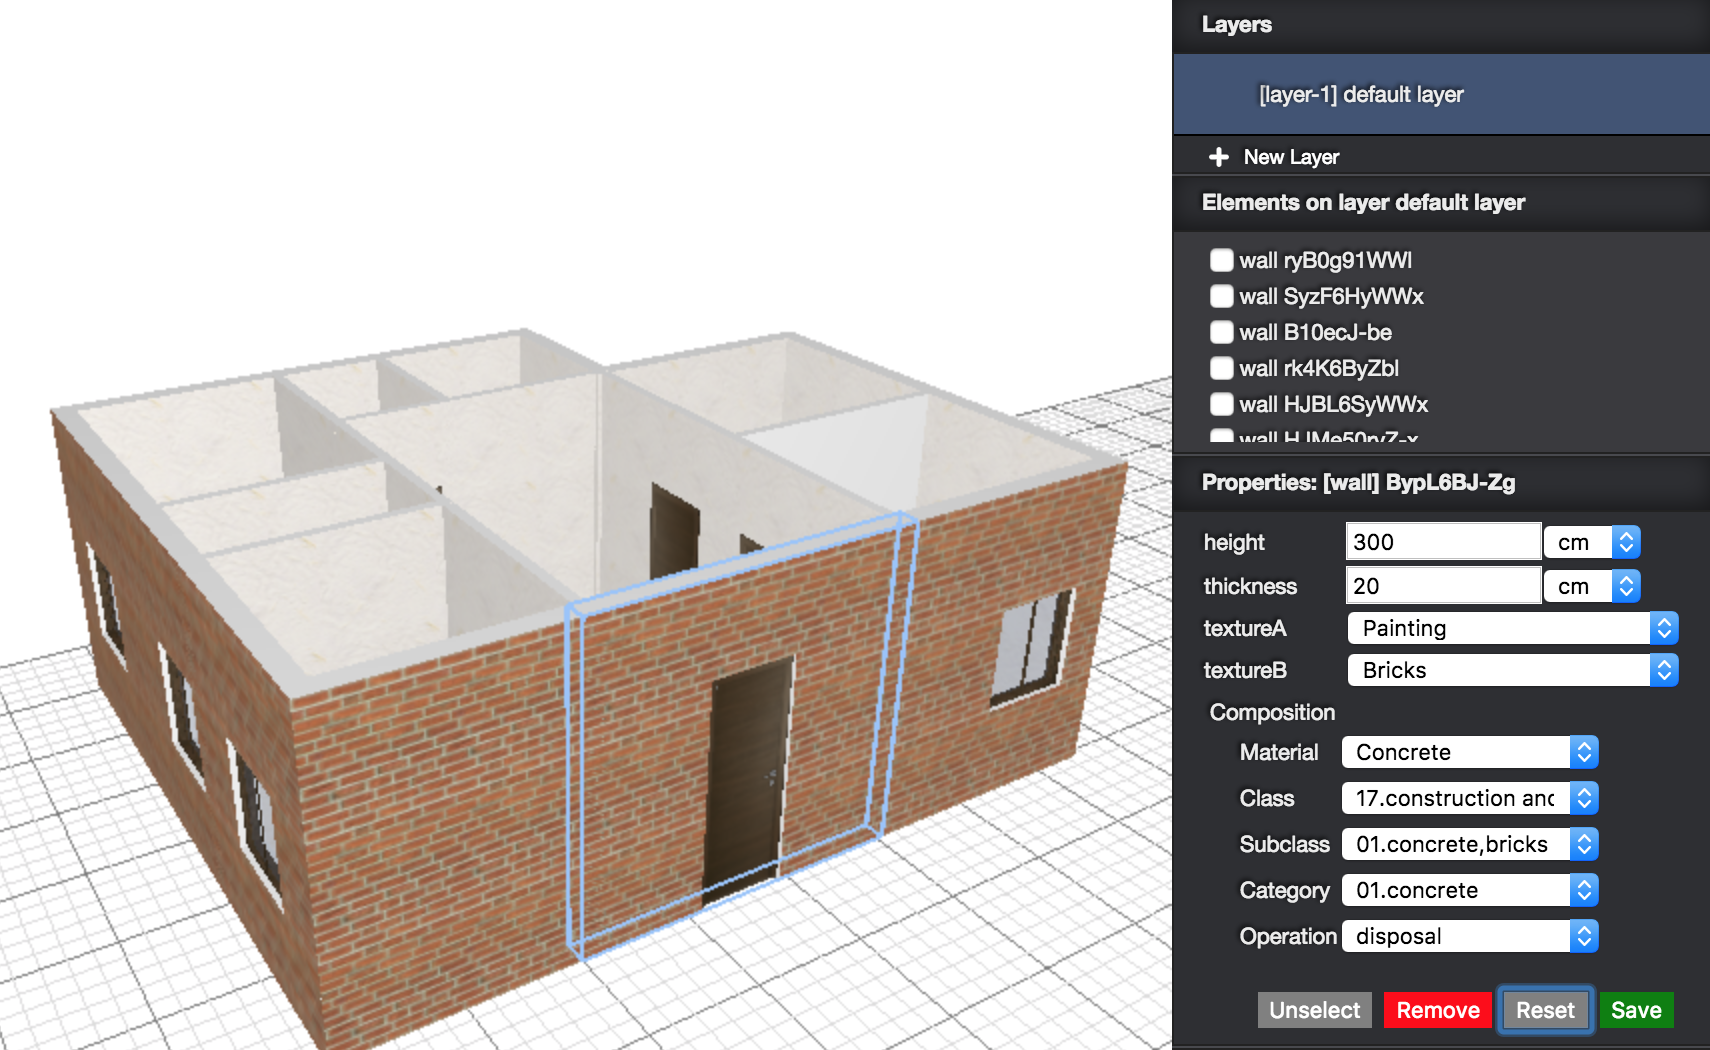
\includegraphics[width=1\linewidth]{images/3d-sel}
   \caption{Vista 3D di un modello per il Deconstruction}
   \label{fig:augmented}
\end{figure}

Un rapporto completo sull'utilizzo BIM su come affrontare una decostruzione di un edificio è fornita da M Galic~\cite{galic2014bim}.
Uno studio sull'uso del BIM come supporto per la progettazione per Deconstruction è svolta da Olugbenga O Akinade~\cite{akinade2015waste}.
In questa configurazione, al contrario di quella usata nel framework \emph{Metior}, la decostruzione deve essere
presa in considerazione a partire dall'inizio della progettazione degli edifici.
\newpage


Il framework \emph{Metior} (dal latino: a \emph{misura} o \emph{stima}),
ha come obiettivo superare tali difficoltà, tramite:
\begin{itemize}
  \item progettazione e realizzazione di un \emph{web service} fornendo un'interfaccia utente semplificata;
  \item memorizzazione un database crescente di \emph{Plugin} che rappresentano un modello per le parti di edificio geometricamente più complesse;
  \item utilizzo un motore geometrico estensibile e affidabile;
  \item l'offerta di integrazioni semantiche flessibili attraverso la specializzazione di (Industry Foundation Classes~\cite{ifc})
        IFC classi associate ai sottosistemi di costruzione e le parti;
\end{itemize}

Considerando ad esempio un progetto che coinvolge la decostuzione di grandi edifici, il processo è
gestito da imprenditori, i quali hanno a disposizione e utilizzano strumenti specifici e hanno delle competenze in questo campo.
La maggiorparte dei materiali di scarto prodotti sono gestiti da geometri provenienti da aziende di piccole o medie dimensioni
o anche da singoli professionisti.
Questo tipo di società necessitano di un sostegno dato da strumenti in cui le complessità,
sia burocratiche che tecniche, anche se nascoste, devono essere correttamente gestite.\\
